\documentclass [a4paper,11pt] {scrartcl}
\usepackage[austrian]{babel}
\usepackage{graphicx}
\author{Robert Lechner}
\title{Java-Codegenerator f{\"u}r DTDs}
\begin{document}
\maketitle
\section{Einleitung}
Das Paket \texttt{dtd2java} besteht aus zwei Teilen:
einem Parser f{\"u}r DTDs (Document Type Definition) und einem Codegenerator,
der aus dem DTD einen XML-Parser mit einem einfachen Modell erzeugt.
In Abbildung \ref{fig:classes} sind die verwendeten Klassen dargestellt.
\begin{figure}[h]
\centerline{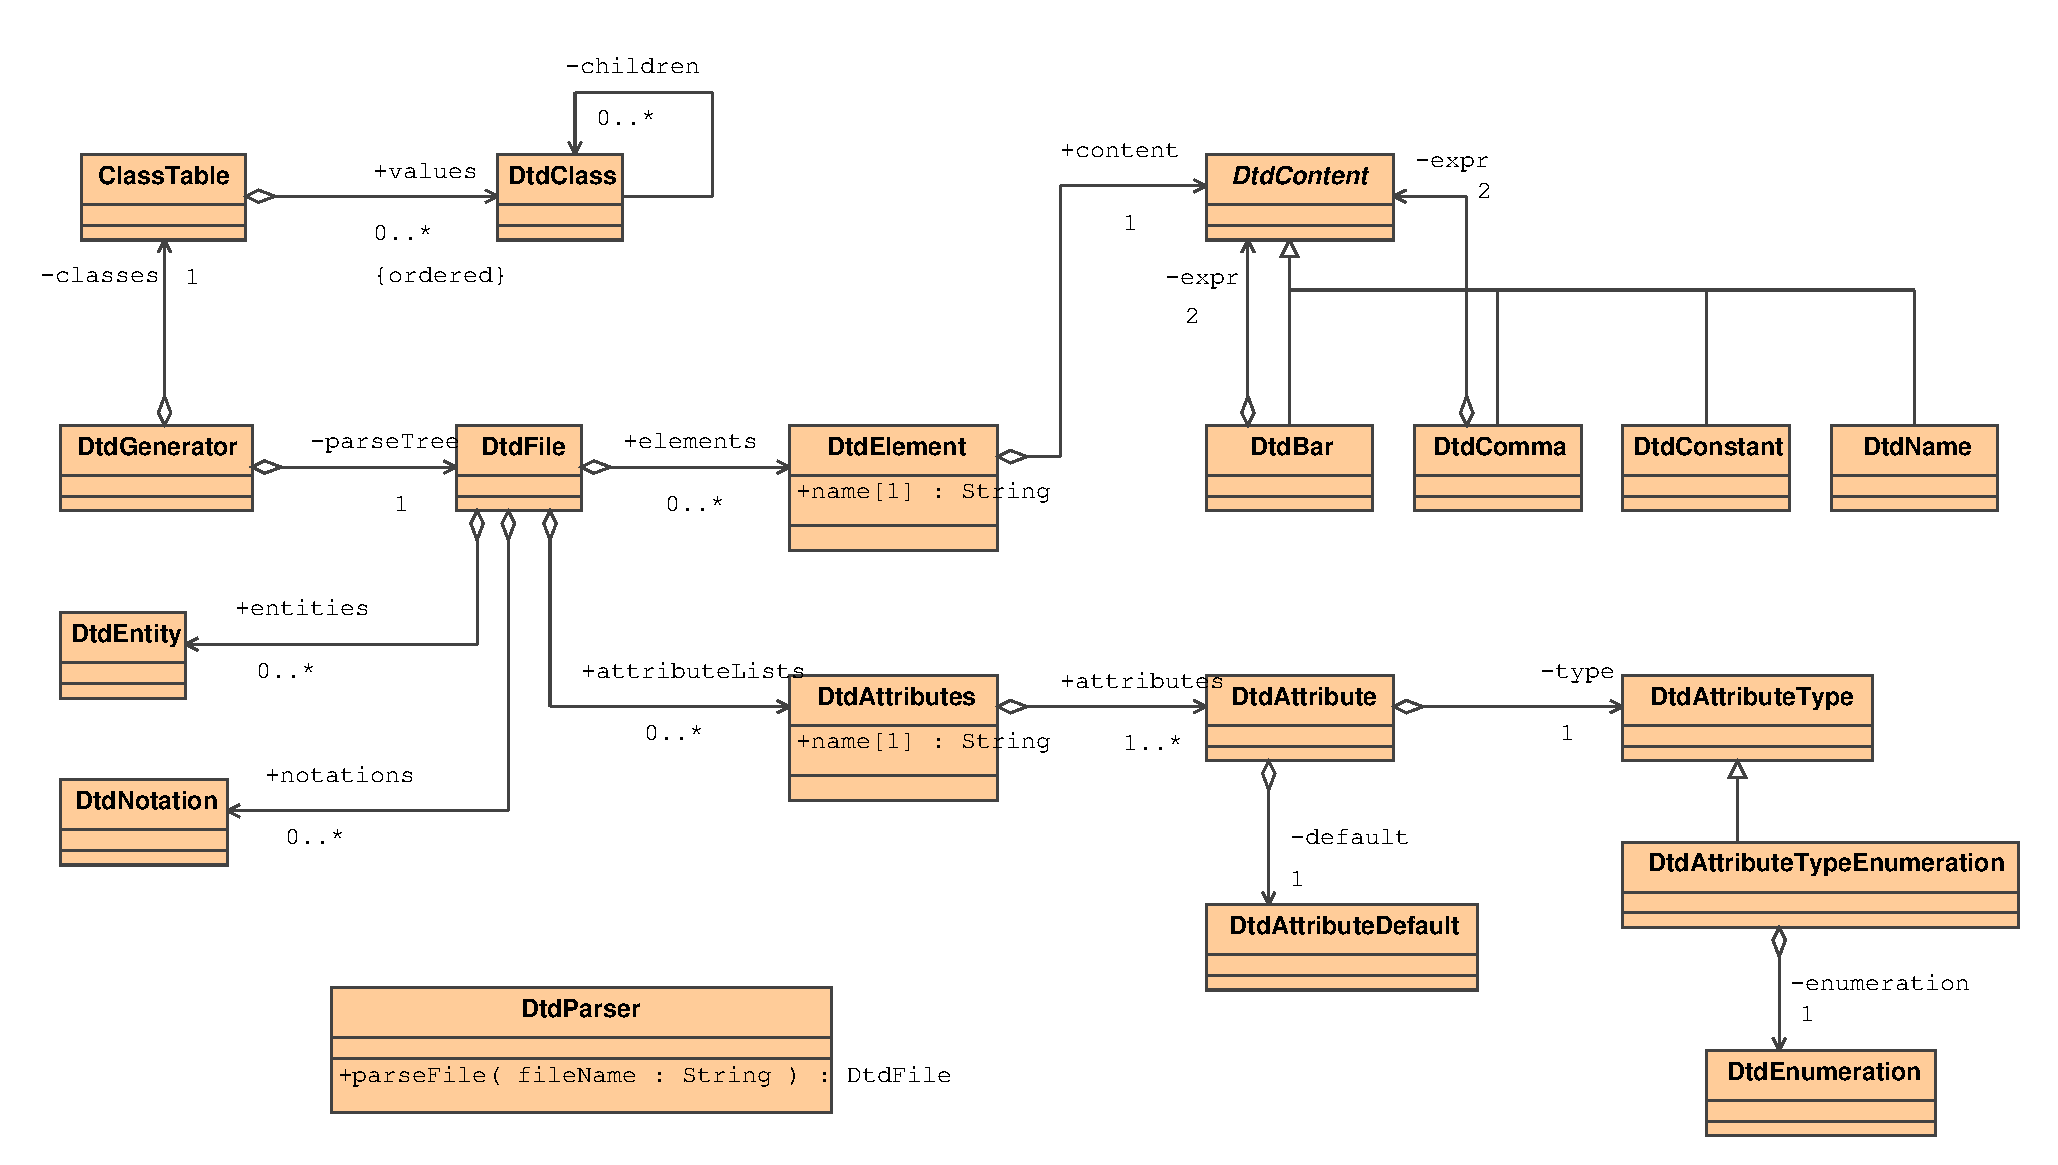
\includegraphics[width=1.2 \linewidth]{classes.eps}}
\caption{{\"U}bersicht {\"u}ber das Paket \texttt{dtd2java}}
\label{fig:classes}
\end{figure}

\newpage
\section{DTD-Parser}
F{\"u}r den DTD-Parser wird der Parsergenerator \textsf{ANTLR} ben{\"o}tigt.
\footnote{ANTLR Translator Generator (http://www.antlr.org)}\\
Zum Lesen eines DTDs ruft man die statische Methode \texttt{DtdParser.parseFile} auf.
Man erh{\"a}lt eine Instanz von \texttt{DtdFile}, welche alle Elemente des DTDs enth{\"a}lt.
Entities werden automatisch expandiert; Attributlisten werden zusammengefasst.

\section{Codegenerator}
\subsection{Aufruf}
Es gibt zwei M{\"o}glichkeiten den Generator zu starten:
\begin{itemize}
\item Erzeugen einer Instanz von \texttt{DtdGenerator} und Aufruf der Methode \texttt{run}.
    Man ben{\"o}tigt dazu aber eine Instanz von \texttt{DtdFile} (siehe oben).
\item Man startet den Generator als Programm:\\
    \texttt{java dtd2java.Main DTD-file Java-package}
\end{itemize}
Der Parameter "`Java-package"', den man in beiden F{\"a}llen ben{\"o}tigt, ist der Name
jenes package, in welchem der erzeugte Code liegen soll. Das Paket wird im aktuellen
Verzeichnis angelegt. Der generierte Code hat die folgenden Eigenschaften:
\begin{itemize}
\item F{\"u}r jedes Element im DTD (\texttt{<!ELEMENT name content >})
    wird eine eigene Klasse generiert. Alle Attribute sind als {\"o}ffentliche Variablen
    direkt zug{\"a}nglich. Der Inhalt des Elements wird in einem allgemeinen Container gespeichert.
\item DTD-Namespaces werden als Java-Packages dargestellt.
\item Der gesamte generierte Code ist \texttt{javadoc}-kompatibel dokumentiert.
\item Es werden alle ben{\"o}tigten Klassen im angegebenen Paket generiert
    $\Rightarrow$ man ben{\"o}tigt zum Ausf{\"u}hren des erzeugten Codes keine
    weiteren Packages (ausgenommen der Java 1.4 Library).
\end{itemize}
Zus{\"a}tzlich werden Dateien f{\"u}r das Tool \textsf{dot} erzeugt.
\footnote{Graphviz (http://www.graphviz.org)}
\newpage
\subsection{erzeugter Code}
Alle Klassen sind von \texttt{DTD\_Container} abgeleitet. {\"U}ber die Methoden \texttt{size}
und \texttt{get} ist der direkte Zugriff auf den Inhalt m{\"o}glich. Mit der {\"o}ffentlichen
Variable \texttt{parent\_\_} kann auf den Vorg{\"a}nger im Baum zugegriffen werden.\\
~\\
In den Unterklassen wird f{\"u}r jedes Attribut des XML-Elements eine {\"o}ffentliche Variable
erzeugt. In der statischen Variable \texttt{xmlName\_\_} steht der vollst{\"a}ndige XML-Name
des Elements. Mit der Methode \texttt{xmlCode} kann der XML-Code erzeugt werden.\\
~\\
Alle Elemente, welche nicht im DTD deklariert wurden, werden als Instanz von
\texttt{DTD\_Generic} gespeichert. Dadurch ist eine Rekonstruktion des XML-Codes
auch bei unbekannten Elementen m{\"o}glich.\\
~\\
Um die Erweiterbarkeit des erzeugten Modells zu gew{\"a}hrleisten, werden alle Instanzen
{\"u}ber eine Factory (\texttt{DTD\_Creator}) erzeugt. Zur Demonstration dient das folgende Beispiel:
~\\[4ex]
\begin{minipage}{\linewidth}
\textbf{XML-Element:}
\begin{verbatim}
package test_model;
import org.xml.sax.*;

public class E9 extends DTD_Container
{
    ...
}
\end{verbatim}
\end{minipage}
~\\[4ex]
\begin{minipage}{\linewidth}
\textbf{Factory:}
\begin{verbatim}
package test_model;
import org.xml.sax.*;

public class DTD_Creator
{
  public DTD_Container create( String qName, Attributes attrs )
  {
    ...
    if(qName.equals("E9"))  return new E9(attrs);
    ...
    return new DTD_Generic(qName, attrs);
  }
}
\end{verbatim}
\end{minipage}
~\\[4ex]
\begin{minipage}{\linewidth}
\textbf{eigenes Element:}
\begin{verbatim}
package test_application;
import test_model.*;
import org.xml.sax.*;

public class MyE5 extends E5
{
    public MyE5( Attributes attrs )
    {
        super(attrs);
    }

    ...
}
\end{verbatim}
\end{minipage}
~\\[4ex]
\begin{minipage}{\linewidth}
\textbf{eigene Factory:}
\begin{verbatim}
package test_application;
import test_model.*;
import org.xml.sax.*;

public class MyFactory extends DTD_Creator
{
    public DTD_Container create( String qName, Attributes attrs )
    {
        if( qName.equals(E5.xmlName__) )
        {
            return new MyE5(attrs);
        }
        return super.create(qName, attrs);
    }
}
\end{verbatim}
\end{minipage}
~\\[4ex]
Der erzeugte Parser wird mit der statischen Methode \texttt{DTD\_Root.parse} aufgerufen.
Dabei kann optional auch eine eigene Factory {\"u}bergeben werden. Im obigen Beispiel
w{\"u}rde der Aufruf wie folgt lauten:
\begin{verbatim}
java.io.File xmlFile = new java.io.File( ... );
DTD_Container root = DTD_Root.parse( xmlFile, new MyFactory() );
\end{verbatim}

\end{document}
